% Lab Writeup for HD Lab
% Adam Reyes, George Wong
% Advanced Lab Fall 2013


\documentclass[paper=a4, fontsize=11pt]{scrartcl} % A4 paper and 11pt font size
\usepackage[left=2.5cm,top=2.5cm,right=2.5cm,bottom=2.5cm]{geometry} 
\usepackage{amsmath}
\usepackage{graphicx}
\usepackage{sectsty}
\usepackage{fancyhdr}
\pagestyle{fancyplain}
\usepackage{parskip}
\usepackage{subcaption}
\usepackage{wrapfig}
\usepackage[english]{babel}
\usepackage{float}
\usepackage{bibentry}
\usepackage {natbib}

\numberwithin{equation}{section}
\numberwithin{figure}{section} 
\numberwithin{table}{section}
%\setlength\parindent{0pt}

\fancyhead[R]{\thepage} 
\fancyhead[L]{Reyes, Wong} 
\fancyhead[C]{Hydrogen-Deuterium Shift} 
\fancyfoot[L]{} 
\fancyfoot[C]{} 
\fancyfoot[R]{} 

\newcommand{\horrule}[1]{\rule{\linewidth}{#1}}

\title{	
The Hydrogen-Deuterium Isotope Shift
\horrule{0.5pt}
\normalfont \normalsize 
\textsc{Advanced Experimental Physics DRAFT Report 2 }
}

\author{Adam Reyes \\ George Wong} % Your name

\date{\normalsize\today} % Today's date or a custom date


\begin{document}
\maketitle



%%%%%%%%%Abstract%%%%%%%%%%%%%%%%%%%%%
\textbf{Abstract:}
Through use of a grating spectrometer, the spectra of both hydrogen and deuterium are measured. Through calculations, the difference in the spectra can be related to the mass difference between a single proton and a proton-neutron pair.

%%%%% INTRODUCTION %%%%%
\section{Introduction}

\subsection{Theory}

The Bohr model of the Hydrogen Atom gives that the allowed energies of
the atom's electron are
\begin{equation}
\label{eq:Hen}
E_n = -\frac{R_E}{n^2}
\end{equation}
Where $R_E$ is the Rydberg energy and $R_E \propto \mu$. Here
$\upsilon$ is the reduced mass of the nucleus and the electron. If we
consider now the isotope of Hydrogen, deuterium, with one neutron it
clearly has a different $\mu$ from plain Hydrogen. So the energy of
the allowed transitions and hence the emission spectrums are
different. The Rydberg formula(eqn \ref{eq:emis}) gives the wavelengths of the emission
spectrum for Hydrogen with an infinitely massive nucleus in terms of
the Rydberg constant $R$.
\begin{equation}
\label{eq:emis}
\frac{1}{\lambda_\infty} = R(\frac{1}{n_1 ^2}-\frac{1}{n_2 ^2})
\end{equation}
Eqn \ref{eq:lamM} gives the the emitted wavelength corrected for the
mass of the nucleus $M$.
\begin{equation}\label{eq:lamM}
\lambda_M = \lambda_{\infty} (1 + \frac{m_e}{M})
\end{equation}
where $m_e$ is the mass of the electron. From this it can be shown
that the mass shift from Hydrogen($M_H$) to Deuterium($M_D$) is
\begin{equation}
\label{eq:mass-shift}
\Delta M = \frac{\Delta \lambda}{\lambda_\infty}\frac{M_D M_H}{m_e}
\end{equation}
difference in reduced masses causes a difference in spectra between hydrogen and deuterium ``isotope shift''

A blazed grating was used in this experiment, which meant that the orientation of the grating (i.e. upwards or downwards) was important and determined the effective brightness of the observed lines. Figure~\ref{fig:diagram1} shows a ``zoomed in'' version of the grating, demonstrating the angled etching on the grating. Light incident from the left (as in the diagram) would necessarily have different intensity in its (e.g.) first order diffraction as compared to light incident from the right.


\subsection{Setup/Apparatus}

A diffraction grating is a reflective material that has had grooves etched into its surface. Incident light reflects off of the surface and, due to interference effects, is refracted by different amounts. Equation~\ref{eq:gratingEqn} gives the relations between incident angle $\alpha$, reflected angle $\beta$, wavelength $\lambda$, and grating resolution $d$.

\begin{equation} \label{eq:gratingEqn}
n \lambda = d ( \sin(\alpha) + \sin(\beta))
\end{equation}

Figure~\ref{fig:diagram1} provides an overhead view of the apparatus.


\begin{figure}[H] \begin{center}
  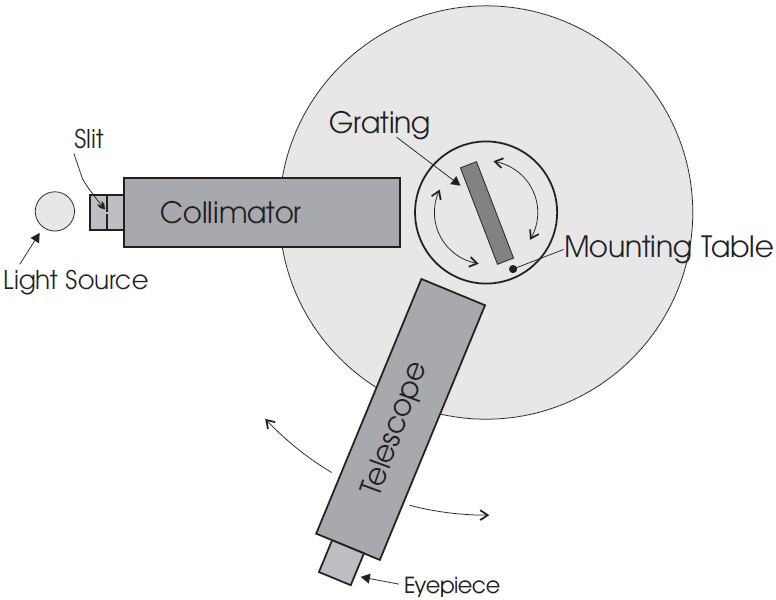
\includegraphics[height=65mm]{diagram1.png}
  \caption{\textbf{Overview of Apparatus} showing relative locations of light source (lamp), collimator with slit, diffraction grating mounted on revolving table, telescope (also on revolving table) and eyepiece.}
  \label{fig:diagram1}
\end{center} \end{figure}


\begin{figure}[H] \begin{center}
  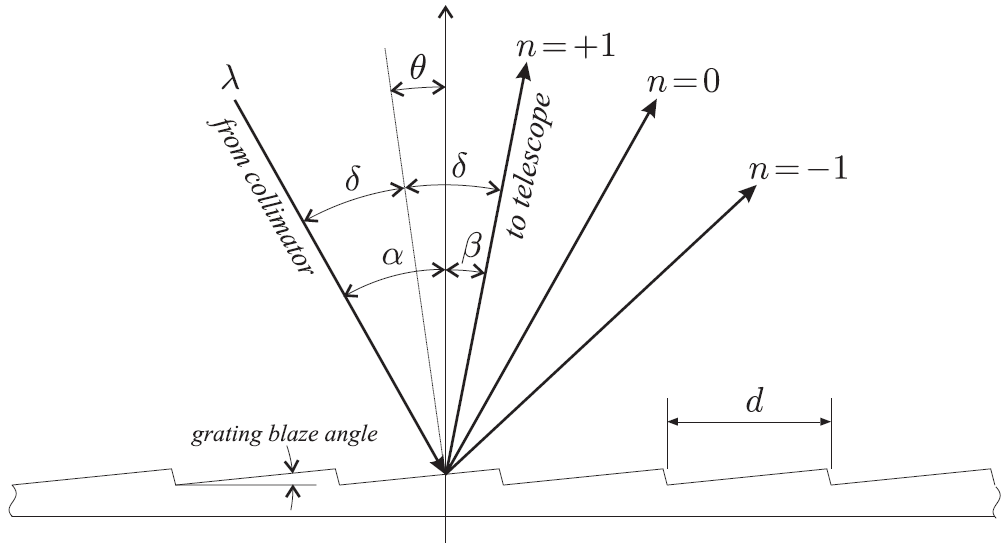
\includegraphics[height=65mm]{grating1.png}
  \caption{\textbf{Micro-scale diagram of diffraction grating} showing grating with grooves and light paths. Angle naming conventions (for $\alpha$, $\beta$, and $\delta$ as well as $n^\mathrm{th}$ order diffraction lines are shown.}
  \label{fig:diagram1}
\end{center} \end{figure}


%%%%% PROCEDURE %%%%%
\section{Procedure}

\subsection{Calibration}

It was important to ensure all parts of the apparatus were focused and adjusted so that the light coming from the slit would diffract off of the grating and enter the telescope at proper angles for viewing.

\begin{enumerate}
\item A two-sided mirror was placed on the mounting table and centered. Its exact location was marked for repeatability.
\item The telescope was then focused to the image of the crosshairs in
  the eyepiece reflected from the mirror.
\item The telescope and mounting table were leveled to each other by
  aligning the horizontal crosshair of the eyepiece to the reflected
  image on both sides of the mirror using the leveling screws of the
  mount and the telescope.
\item The mirror was removed from the central mounting table and the telescope and collimator were brought to be in line with each other.
\item A light was placed behind the slit on the collimator and the distance of the lens in from the slit within the collimator was adjusted until the image of the slit as seen through the eyepiece was as focused as possible.
\item The cross hairs were positioned immediately on the slit and half way up the slit, so as to align the plane of the collimator with that of the telescope/mounting table (already aligned).
\end{enumerate}


\subsection{Angular Alignment}
\label{sec:angal}
Knowledge of the exact measures of angles was very important in this
lab, so the following method was developed to permit precise
measurements of angles. The following assumes the experimenter wishes
to generate a set up with incident angle $\alpha$, between the
collimator and normal incidence to the grating.

\begin{enumerate}
\item The telescope was aligned to normal incidence with the mirror by
  aligning the vertical crosshair of the eyepiece with its reflected image. 
\item With the position of the mount fixed, the telescope was rotated
  by the desired angle $\alpha$.
\item The relative angle of the telescope and mounting table was
  fixed, and the two pieces were moved together until the reflection
  from the slit image was aligned with the vertical crosshair. 
\item At this point, the incident and reflected angles were equal and exactly $\alpha$. The angular position of the mounting table was fixed.
\end{enumerate}

\subsection{Eyepiece Calibration}
\label{sec:eyecal}

In order to make precise angular measurements for this experiment we
used an eyepiece with a thin cross hair that could be moved with a
micrometer screw gauge. The divisions on the gauge had to be
calibrated in order to know what grating angle is swept through as the
screw was turned. This was done by picking two lines separated by as
much arc length as could fit in the view of the eyepiece. This angle
was then measured using the protractor on the spectrometer, then
measured using the eyepiece gauge. It was then determined that one
eyepiece unit corresponds to $0.0023\pm0.0001^{\circ}$

\subsection{Measurement of Spectra}
\label{sec:specmes}
In this section, we actually measure the spectra of the light (emission spectra) as a function of angle. The following procedure was performed with both the provided Sodium and Hydrogen-Deuterium lamps; however, it would be exactly the same for any lamp/source.

\begin{enumerate}
\item An angle of incidence $\alpha$ was obtained using the procedure
  outlined in~\ref{sec:angal}.
\item A light source (lamp) was placed before the slit and was covered with a blackout sheet, so as to completely darken the room.
\item The telescope was rotated from the zeroth order reflection until a line was visible. At this point, the cross hairs were brought to rest directly on the center of the line. The relative change in angle off zeroth order is noted.
\item The above step was repeated until the telescope could not be physically rotated any further.
\end{enumerate}




%%%%% DATA + ANALYSIS/RESULTS %%%%%
\section{Data \& Analysis}

The angular divisions on the rotation table came with the smallest unit of $1/3^\circ$. For each of our measurements not involving the fine-adjustment eyepiece, our recorded values were to a precision of $1/30^\circ$, or $1/10$ of the smallest marked measure.

One gauge marking on the fine-adjustment eyepiece was found to be: \\
$1$ guage $= 0.0023\pm0.0001$ degrees.

\begin{table}[H]
\centering
\caption{\textbf{Hydrogen/Deuterium Spectrum Lines} taken with angle of incidence $\alpha = 45^\circ$ and use of fine-adjustment knob. }
\begin{tabular}{ || c | c c c c c || }
  \hline
  \hline
  line & degrees & $(\frac{1}{3})^\circ$ & $(\frac{1}{30})^\circ$ & left line (gauge)  & right line (guage) \\
  \hline
  zeroth & $376$ & $2$ & $8$ & $0$ & n/a \\
  red & 346 & $1$ & $2$ & 1.5 & 5.7 \\
  blue & 352 & 2 & 8 & 18.9 & 23 \\
  \hline
  \hline
\end{tabular}
\label{table:hd45}
\end{table}

\vspace{1.5em}

To determine the wavelengths corresponding to various lines, Equation~\ref{eq:gratingEqn} was rewritten with the value $K$ as the grating resolution:
\begin{equation}
\label{eq:wavelengthEqn}
n \lambda = \dfrac{1}{K} \left( \sin(\alpha) + \sin(\beta) \right)
\end{equation}

 Because the grating used had a resolution of $600$ grooves/mm, $K=600$. The angle of incidence $\alpha$ corresponded to $45^\circ$ or $60^\circ$, depending on data set. The angle $\beta$ was given by the angle difference between the zeroth order and the measured line. The order of the line $n$ (an integer) was either known from mere sight recognition or adjusted until the wavelength value made sense (was in the visible light range).

Table~\ref{table:hd-calculated} gives the calculated wavelength values.

\begin{table}[H]
\centering
\caption{\textbf{Hydrogen/Deuterium Line Wavelengths} given in
  (nm). $\lambda_{\infty}$ values given account for 100 nm systematic shift. }
\begin{tabular}{ || c | c c c c || }
  \hline
  \hline
  line & wavelength (left) [nm] & wavelength (right) [nm] & $\Delta
  \lambda$ [nm] & $\lambda_{\infty}$ [nm] \\
  \hline
  red & 761.75 & 761.48 & 0.27 & 656\\
  blue & 579.82 & 579.56 & 0.26 & 486\\
  \hline
  \hline
\end{tabular}
\label{table:hd-calculated}
\end{table}

\vspace{1.7em}


In an attempt to eliminate systematic error, the Sodium (Na) spectrum was also measured. The calculated wavelength values for Sodium were compared to the accepted Sodium spectrum wavelengths, which has lines at $589.0$ and $589.6$ nm. The difference between accepted and calculated values was compared for first and second order diffraction lines, and a rough linear relationship between degree and offset was established.

\begin{table}[H]
\centering
\caption{\textbf{Sodium Spectrum Lines} taken with angle of incidence $\alpha = 60^\circ$ without use of fine-adjustment eyepiece }
\begin{tabular}{ || c | c c c || }
  \hline
  \hline
  line & degrees & $(\frac{1}{3})^\circ$ & $(\frac{1}{30})^\circ$  \\
  \hline
  zeroth & $361$ & $2$ & $8$  \\
  first (left) & 337 & $2$ & $1$  \\
  first (right) & 337 & 2 & 1 \\
  second (left) & 317 & 0 & 2 \\
  second (right) & 317 & 0 & 1 \\
  \hline
  \hline
\end{tabular}
\label{table:sodium60}
\end{table}

\begin{table}[H]
\centering
\caption{\textbf{Sodium Spectrum Lines} taken with angle of incidence $\alpha = 45^\circ$, making use of fine-adjustment eyepiece }
\begin{tabular}{ || c | c c c c c || }
  \hline
  \hline
  line & degrees & $(\frac{1}{3})^\circ$ & $(\frac{1}{30})^\circ$ & left line (gauge)  & right line (guage) \\
  \hline
  zeroth & $376$ & $2$ & $8$ & $0$ & n/a \\
  first & 348 & $2$ & $1$ & 0 & 10.7 \\
  second & 327 & 0 & 0 & 0 & 18 \\
  third & 306 & 2 & 6 & 0 & 28.8 \\
  \hline
  \hline
\end{tabular}
\label{table:sodium45}
\end{table}

Using the same formula as given above in Equation~\ref{eq:wavelengthEqn}, the corresponding wavelengths of the Na line were found and are presented in Table~\ref{table:na-wavelength}.

\begin{table}[H]
\centering
\caption{\textbf{Sodium Line Wavelengths} calculated }
\begin{tabular}{ || c | c c c || }
  \hline
  \hline
  line & $n\lambda$ (nm) & order & wavelength (nm)  \\
  \hline
  left & 697.4 & 1 & 697.4 \\
  right & 696.8 & 1 & 696.8 \\
  left & 1321.3 & 2 & 660.7 \\
  right & 1320.1 & 2 & 660.1 \\
  left & 1883.9 & 3 & 628.0 \\
  right & 1882.1 & 3 & 627.4 \\
  \hline
  average $\Delta\lambda$ & $--$ & $--$ & 0.6 \\
  \hline
  \hline
\end{tabular}
\label{table:na-wavelength}
\end{table}

The accepted wavelengths for the sodium spectra lines are given in Table~\ref{table:na-accepted}.

\begin{table}[H]
\centering
\caption{\textbf{Accepted Sodium Spectrum Wavelengths}}
\begin{tabular}{ || c | c || }
  \hline
  \hline
   & $\lambda$ [nm] \\
  \hline
  ``left'' & $588.9950$ \\
  ``right'' & $589.5924$ \\
  \hline
  $\Delta$lines & $0.5974$ \\
  \hline
  \hline
\end{tabular}
\label{table:na-accepted}
\end{table}

A comparison of the experimentally recovered wavelength values versus accepted values yields two noteworthy observations: (1) experimental wavelengths were off from expected values by $\approx 100 - 170$ nm and (2) the difference in wavelength between the two lines ($\Delta\lambda_1\lambda_2$) in experimental data was found to be consistently $0.6$nm, a value which perfectly corresponds to its accepted counterpart.

Due to the correlation between experimental and accepted values for $\Delta \lambda_1 \lambda_2$, it was decided that the experimental $\Delta \lambda$ values were deemed usable.

\vspace{1.2em}

\hrule
\vspace{0.7em}



\begin{table}[H]
\centering
\caption{\textbf{Hydrogen/Deuterium Spectrum Lines} taken with angle of incidence $\alpha = 60^\circ$ and no use of fine-adjustment knob. }
\begin{tabular}{ || c | c c c || }
  \hline
  \hline
  line & degrees & $(\frac{1}{3})^\circ$ & $(\frac{1}{30})^\circ$  \\
  \hline
  zeroth & $351$ & $0$ & $8$  \\
  faint purple & 333 & $1$ & $8$  \\
  bright purple & 332 & 2 & 2 \\
  faint purple & 332 & 1 & 7 \\
  bright green-blue & 330 & 2 & 0 \\
  very faint green-blue & 330 & 0 & 8 \\
  very faint green-blue & 330 & 0 & 1 \\
  faint green & 328 & 2 & 8 \\
  very faint green & 328 & 1 & 2 \\
  bright red & 325 & 2 & 7 \\
  faint red & 324 & 2 & 3 \\
  very bright red & 324 & 1 & 1 \\
  very faint purple & 318 & 1 & 4 \\
  bright purple & 316 & 2 & 6 \\
  faint purple & 316 & 1 & 9 \\
  bright blue-green & 313 & 0 & 7 \\
  very faint blue-green & 312 & 1 & 2 \\
  very faint blue-green & 312 & 0 & 1 \\
  faint purple & 309 & 2 & 9 \\
  faint purple & 309 & 0 & 8 \\
  faint red & 304 & 0 & 7 \\
  purple & 301 & 2 & 6 \\
  extremely faint purple & 301 & 1 & 7 \\
  very bright red & 301 & 1 & 2 \\
  bright blue & 296 & 1 & 2 \\
  extremely faint blue & 295 & 0 & 8 \\
  \hline
  \hline
\end{tabular}
\label{table:hd60}
\end{table}


In addition to the data reproduced in the above tables, another group of angles at which spectral lines were observed was taken and is reproduced in Table~\ref{table:hd60}. Unfortunately, these data proved to be wrought with error and quantitative analysis proved meaningless. For completeness sake, they are still presented. At the very least, the recorded apparent colors of the lines in the spectra can be used to qualitatively classify the spectrum.

Potential sources of this error are discussed below in the \textbf{Conclusion} section.

\vspace{1.5em}
\hrule
\vspace{1.7em}

To calculate the actual difference in mass, the Rydberg formula for reduced mass was used. Equation~\ref{eq:rydberg-rm} was considered in determining the inverse proportionality of wavelength to reduced mass, as in Equation~\ref{eq:inverse-prop}.

\begin{equation}
\label{eq:rydberg-rm}
E_i - E_f = \dfrac{hc}{\lambda} = \dfrac{\mu_X Z^2 e^4}{\left( 4 \pi \epsilon_0 \right)^2 2 \hbar^2} \left[ \dfrac{1}{n^2_f} - \dfrac{1}{n_i^2} \right]
\end{equation}

\begin{equation}
\label{eq:inverse-prop}
\dfrac{1}{\lambda} \propto \mu
\end{equation}

This leads to the following expression for the wavelengths emitted by
a finite mass nucleus
\begin{equation}
  \label{eq:inf}
  \lambda_M = \lambda_{\infty}(1-m_e/M)^{-1}
\end{equation}
This is in contradiction with the expression given in the
writeup\cite{writeup},
\begin{equation}
  \label{eq:writeup}
  \lambda_M = \lambda_{\infty}(1+m_e/M)
\end{equation}
Equation(\ref{eq:inf}) leads to the following expression for the mass
ratio of Deuterium to Hydrogen
\begin{equation}
  \label{eq:ratio}
  \frac{M_D}{M_H} =
  \left[
    \frac{1+m_e/M_H}{1-\Delta\lambda/\lambda_{\infty}}-1
  \right]^{-1}
\end{equation}
Using the data from Table~\ref{table:hd-calculated} we get
\begin{table}[h]
  \centering
  \begin{tabular}{|| c | ccc ||} \hline \hline
    $\Delta \lambda$ [nm] & $M_D/M_H$ & $M_D$ [Mev/c$^2$] & M$_n$[Mev/c$^2$]\\ \hline
    0.26 & 1.70 & 1595.05 & 654.56 \\
    0.27 & 1.91 & 1792.09 & 851.59 \\ \hline \hline
  \end{tabular}
  \caption{Mass ratio calculations}
  \label{tab:ratio}
\end{table}
We can get the neutron mass by subtracting the nuclear binding energy
of Deuterium. To do these calculations we use 
\begin{align}
\begin{split}
  \label{eq:things}
  \centering
  m_e/M_H &= 1836.12\\
  M_H & = 938.27 MeV/c^2\\
  \Delta E_{binding} & = 2.23 MeV
\end{split}
\end{align}

% From this, the relation between wavelengths and masses is found, given in Equation~\ref{eq:wavelength-masses}, wherein the 

% \begin{equation}
% \label{eq:wavelength-masses}
% \dfrac{\lambda_H - \lambda_D}{\lambda_{\infty}} = \dfrac{1-M_H / M_D}{1+M_H/m}
% \end{equation}


% From Equation~\ref{eq:mass-shift}, we can calculate the ratio of the
% nuclear masses of Hydrogen and Deuterium.

% Equation~\ref{eq:deltaMass} gives the mass ratio with $m_e$ the mass of an electron, and $\Delta \lambda$ is the difference in wavelength between the Hydrogen and Deuterium isotope spectrum lines.

% \begin{equation}
% \label{eq:deltaMass}
% \frac{M_D}{M_H} =
% \left[
% 1 - \frac{\Delta \lambda}{\lambda_{\infty}}
% \left(
% 1 + \frac{M_H}{m}
% \right)
% \right]^{-1}
% \end{equation}

% $TODO$

% $\Delta M = \dfrac{ 0.27 \, \mathrm{nm} } { \lambda_\infty } \dfrac{ M_D M_H} { 0.51 \, \mathrm{MeV/C}^2 }$

% $\Delta M = \dfrac{0.26 \, \mathrm{nm} } { \lambda_\infty } \dfrac{M_D M_H} { 0.51 \, \mathrm{MeV/C}^2}$

% So the average $\Delta M = TODO$


% $TODO$

% Given that the mass of the proton is 1836.12 times the mass of the electron, compute the mass of the
% neutron or rather, the difference between the mass of the deuteron and the proton. The neutron mass
% can be obtained from M by observing that the binding energy of the deuteron is 2.23 MeV.


\section{Conclusion}

Quantitatively, we found $\Delta M$, the difference in mass between Hydrogen and Deuterium to be $TODO$. Further, from this value, we found the mass of a neutron to be $TODO$. This compares to the accepted mass of a neutron, which is $940 \, \mathrm{MeV/C}^2$.


It was important to consider exactly what was being observed during the course of the experiment. In the case of the data taken for Table~\ref{table:hd60}, it turned out that many of the observed lines were artifacts or some other unknown phenomenon, and therefore were useless in qualitative analysis.

Performing the sodium calibration was massively useful as it allowed us to verify our angle finding/setting methodologies. Further, it allowed us to qualitatively get a feel for what angular distances corresponded to what wavelength differences. Each of the observed lines in the Hydrogen-Deuterium spectra was, upon close examination, actually a set of two lines. This is an entirely expected result, as the difference in masses between the Hydrogen and Deuterium in the samples should/would split each observable line into two.

Ideally, a comparison of the spectra of both pure Hydrogen and the Hydrogen-Deuterium mixture would be observed; however, due to time constraints and the poor quality of available Hydrogen lamps, this experiment was not performed. \\

One of the major sources in error came from our inability to precisely determine the angle of incident of light on the mirror. While the method for determining the angle of incidence given above is geometrically sound, precision was difficult to attain. Further, the static friction between the two rotating surfaces was relied upon during the initial setup and there was no way to ensure that the two plates did not move relative to each other unintentionally.

Of course, the above error is relatively insignificant as compared to uncertainty in degree measures for the locations of the emission lines. Two eyepieces were used because the thickness of the crosshairs on one of the eyepieces was larger than the spacing between the lines in some cases. \\

Over the course of performing the experiment, it was found that many of the procedures were difficult or impossible to perform well due to the condition of the apparatus. Precise angular measurements were nearly impossible due to the amount of light needed in order to see both the reticule and the line. Overall, the alignment of the device (in terms of collimator, mounting table, and telescope) was next-to-impossible due to misalignment of the mirror/grating in the vertical plane. Also, the grating seemingly had several scratches on it and was overall in bad condition. For the angles measured to yield more precision in the calculations of wavelength, a grating with a higher resolution might be used.

A particularly troublesome part of the experiment was actually determining where the spectrum lines actually were. The necessitated low-light condition of the room made the crosshairs very difficult to view, and so precise alignment (especially at such a fine visual resolution) was incredibly difficult.

As was noted in the \textbf{Data \& Analysis} section, there was a discrepancy between the measured and accepted wavelength values for spectral lines in Sodium that ranged from $100$ to $\approx 170$ nm. Unfortunately, the reasoning for this remains undetermined. Potential explanations include: defects in the grating causing uneven diffraction of light, defects in telescope optics causing light to bend in unanticipated ways, light incident to the diffraction grating from other sources in the room, and impurities in the original lamp source.




\bibliographystyle{plain}
\bibliography{references}




\end{document}